\subsection{Исследование неподвижных точек на устойчивость}

Пусть задана динамическая система с непрерывным временем
\begin{equation}\label{eq:common_continuous_system}
        \dot u = f(u),\; u \in U \subseteq \R^n,\; f:U\rightarrow\R^n.
\end{equation}
Пусть $u^*$~--- неподвижная точка системы \ref{eq:common_continuous_system}, $J(u^*)$~--- матрица Якоби функции $f(u)$ в точке $u^*$. $n_+,\; n_0,\; n_-$~--- количество собственных значений матрицы $J(u^*)$, учитывая кратность, с положительной, нулевой и отрицательной вещественной частью соответственно.

\begin{definition}
        Положение равновесия $u^*$ динамической системы \ref{eq:common_continuous_system} называется гиперболическим, если $n_0 = 0$ (не существует собственных значений, расположенных на мнимой оси). Гиперболическое положение равновесия называется гиперболическим седлом, если $n_+\cdot n_- \neq 0$.
\end{definition}
\begin{theorem}[А.~M.~Ляпунов, А.~Пуанкаре]
        Пусть $u^*$~--- гиперболическое положение равновесия системы \ref{eq:common_continuous_system}. Пусть $n_+,\; n_-$~--- число собственных значений $J(u^*)$ с положительной и отрицательной вещественной частью соответственно. Тогда, если $n_+ = 0$, то положение равновесия $u^*$ асимптотически устойчиво, если $n_+ > 0$, то неустойчиво. \cite[стр.~107]{bratus10}
\end{theorem}

Воспользуемся теоремой Ляпунова--Пуанкаре. Для этого выпишем матрицу Якоби изучаемой системы \ref{eq:short_continuous_system}, предварительно зафиксировав параметр $\gamma = 1$.
$$
        J =
        \begin{pmatrix}
                -\alpha\ln u-\alpha-\beta v & -\beta u\\
                \frac{v}{1+v} & -1 + \frac{u}{(1 + v)^2}
        \end{pmatrix}
$$
Рассмотрим значения якобиана в найденных ранее неподвижных точках $A(0,\;0)$ и $B(1,\;0)$.

Ввиду наличия логарифмического слагаемого значение якобиана в точке $A$ не определено. Рассмотрим значение якобиана в некоторой точке $A_\varepsilon(\varepsilon, 0)$:
$$
        J(A_\varepsilon) =
        \begin{pmatrix}
                -\alpha\ln\varepsilon & -\beta\varepsilon\\
                0 & -1 + \varepsilon
        \end{pmatrix}
$$
Получаем собственные значения $\lambda_1 = -\alpha - \ln\varepsilon$ и $\lambda_2=-1+\varepsilon$. Устремляя $\varepsilon$ к нулю, получаем, что $\lambda_1 > 0$, а $\lambda_2 < 0$. Значит точка $A$ является седлом.

Рассмотрим теперь значение якобиана в точке $B$:
$$
        J(B) =
        \begin{pmatrix}
                -\alpha & -\beta\\
                0 & 0
        \end{pmatrix}
$$
Собственными значениями матрицы $J(B)$ являются $\lambda_1 = -\alpha < 0$ и $\lambda_2 = 0$. Данное положение равновесия является устойчивым. Но при этом для данной точки характерна бифуркация "<седло-узел">, возникающая при прохождении парамером $\gamma$ значения $1$.

\begin{figure}[h]
        \centering
        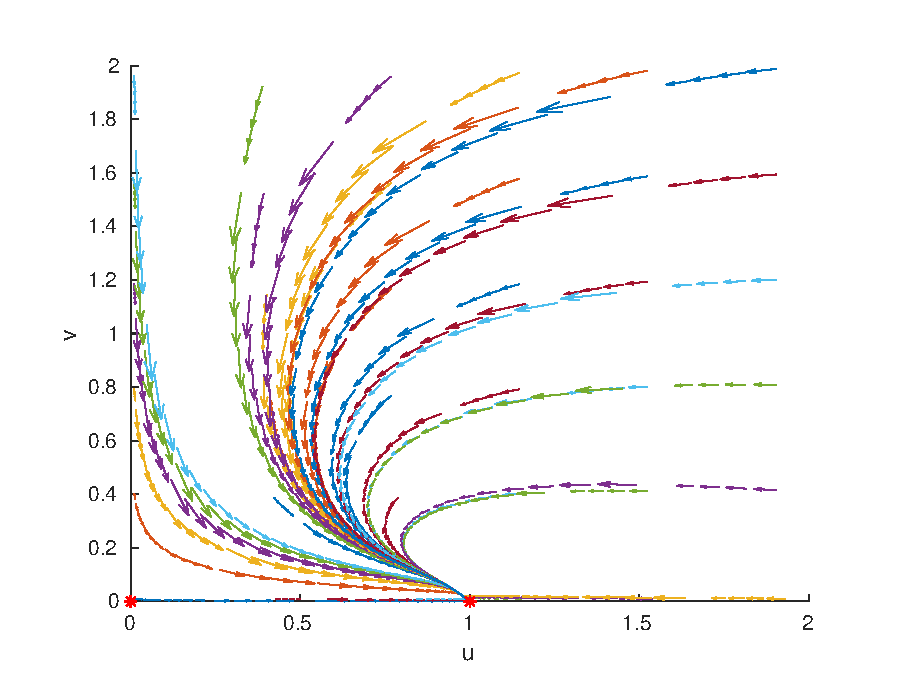
\includegraphics[width=0.8\linewidth]{continuous_system/stability_of_fixed_points/common.eps}
        \caption{Фазовый портрет системы \ref{eq:short_continuous_system}. $\alpha = \beta = \gamma = 1$.}
\end{figure}

\begin{figure}[h]
        \centering
        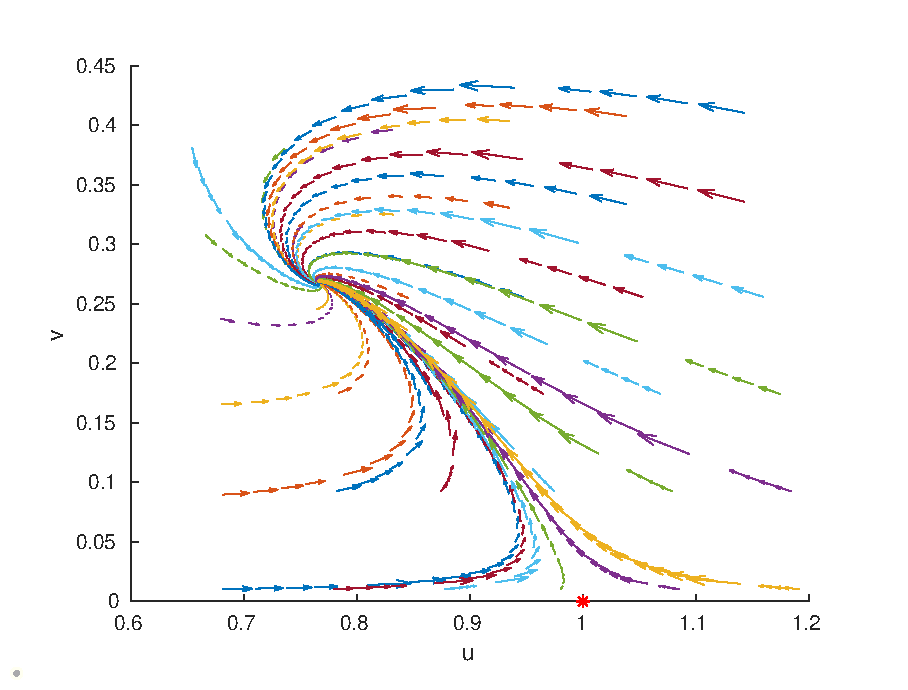
\includegraphics[width=0.8\linewidth]{continuous_system/stability_of_fixed_points/r0-5.eps}
        \caption{Изменение состояния системы при $\gamma < 1$.}
\end{figure}

\begin{figure}[h] 
        \centering
        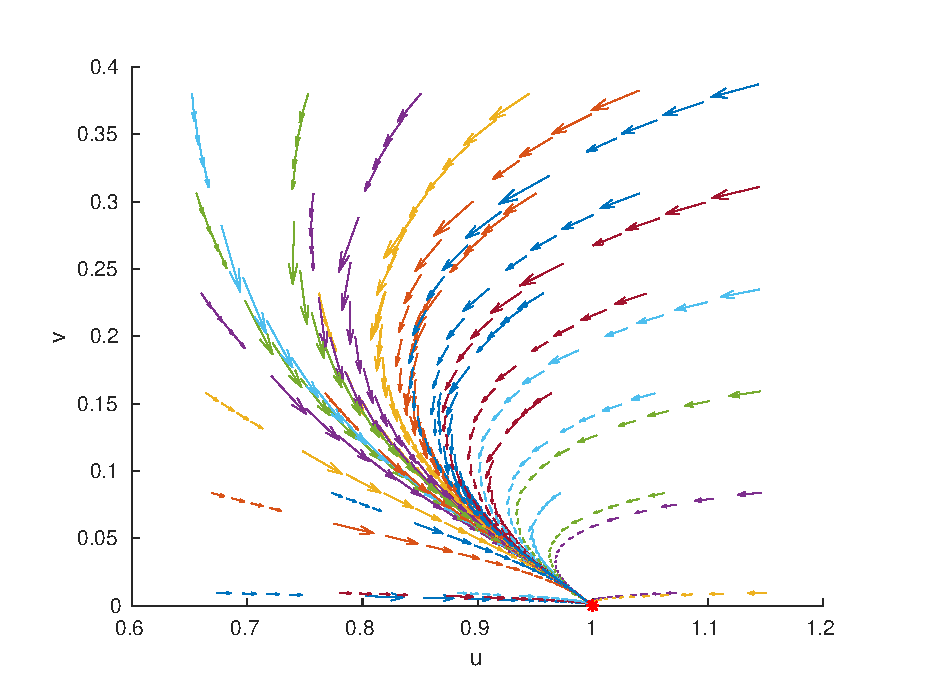
\includegraphics[width=0.8\linewidth]{continuous_system/stability_of_fixed_points/r1-5.eps}
        \caption{Изменение состояния системы при $\gamma > 1$.}
        \label{img:bifurcation}
\end{figure}

На Рис.~\ref{img:bifurcation} так же видно появление узловой точки при $\gamma < 1$, которую мы не будем рассматривать в силу фиксации параметра $\gamma$. Приводить параметрический портрет системы не  имеет смысла, так как в нашем случае есть только одно состояние. 